\documentclass[]{article}
\usepackage[utf8]{inputenc}
\usepackage[spanish]{babel}
\usepackage{graphicx}
\usepackage{color}
\usepackage[usenames,dvipsnames,svgnames,table]{xcolor}
\usepackage{hyperref}
\usepackage{url}
\usepackage{listings}
\hypersetup{
	colorlinks   = true,
	citecolor    = gray,
	urlcolor     = darkgray,
	linkcolor	 = darkgray
}

%opening
\title{Sistemas Inteligentes para la Gestión en la Empresa\\-\\Práctica 2: Deep Learning para multi-clasificación}
\author{Carlos Cobos Suárez\\Adrián Morente Gabaldón}

\begin{document}

\maketitle
\newpage
\tableofcontents
\newpage

\section{Introducción}

En este proyecto vamos a realizar diversas aproximaciones al tratamiento de técnicas de \textbf{aprendizaje profundo} con el lenguaje \textbf{\textit{R}}. Tras ponernos en situación con los fundamentos teóricos necesarios para entender el desarrollo realizado, comentaremos las soluciones pensadas y las que finalmente se hayan implementado; realizando después una discusión de los resultados obtenidos.\\

El conjunto de datos (o \textit{dataset}) que utilizaremos se corresponde con el de \textbf{\textit{PetFinder.my Adoption Prediction}}, y podemos encontrarlo en la plataforma \href{https://kaggle.com}{Kaggle} \cite{petfinder-dataset}. Los datos contenidos clasifican un histórico de perros y gatos alojados en centros de adopción de animales, con diversas características y almacenando el \textbf{tiempo de adopción} de cada una de estas mascotas.\\

El trabajo a desarrollar en este proyecto versa sobre el \textbf{entrenamiento de modelos de predicción} que, a partir de imágenes o de un conjunto de características de animales, clasifiquen éstos por tiempo de adopción. Para dicha clasificación, utilizaremos \textbf{cinco categorías} (las cuales se ordenan según el tiempo de adopción en orden ascendente). Lógicamente, la finalidad del trabajo será la de obtener la mejor precisión general posible, para lo que utilizaremos distintos modelos basados en \textbf{aprendizaje profundo}.\\

Dado que para el entrenamiento se dispone de un gran conjunto de datos ya clasificado, realizaremos algún \textbf{histograma}, lo que trata de un gráfico de barras que muestra el cardinal del conjunto de datos de cada una de las distintas categorías mencionadas.\\

Por otro lado, realizaremos también un \textbf{trabajo de investigación} relacionado con la aplicación de \textbf{técnicas de binarización}, planteando un marco teórico y comentando las distintas posibilidades que ofrecen.

\section{Fundamentos teóricos}

	Para entender tanto la finalidad del proyecto como los pasos realizados para su compleción, debemos ubicarnos en un marco teórico apropiado. Para empezar, antes de abordar la temática relacionada con el \textbf{aprendizaje profundo}, debemos hablar del \textbf{aprendizaje automático} y las técnicas más destacadas para su puesta en uso, como pueden ser las \textbf{redes neuronales} de diversos tipos.
	
	\subsection{Redes neuronales}
	
		Sabemos que la unidad básica de una red neuronal es, lógicamente, la \textbf{neurona}; cuya función es recibir unos datos de entrada, procesarlos mediante algunas operaciones matemáticas, y producir una salida.\\
		
		Estas entradas pueden provenir de la entrada al sistema o de la salida por parte de otras neuronas. Además, el número de éstas es variable, como podemos ver en la figura \ref{neuron}, donde se visualiza un ejemplo de neurona con dos entradas y una salida \cite{introduction-neural-networks}.\\
	
		\begin{figure}[h]
			\centering
			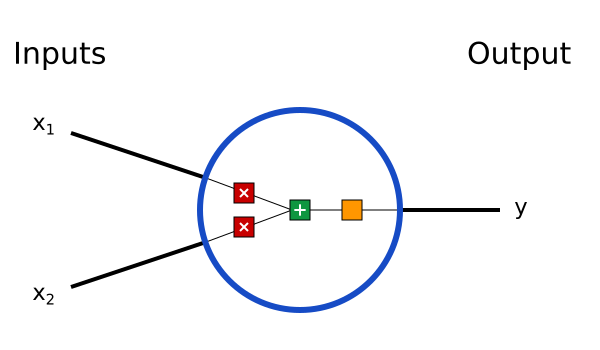
\includegraphics[width=0.5\textwidth]{./img/neuron}
			\caption{Neurona simple con dos entradas y una salida.}
			\label{neuron}
		\end{figure}
	
		Como se podría esperar a raíz de su nombre, sabiendo lo que es una neurona, podemos esperar que una \textbf{red neuronal} sea un conjunto conectado de varias neuronas. Podemos ver un ejemplo en la figura \ref{neural-network}.\\
		
		\begin{figure}[h]
			\centering
			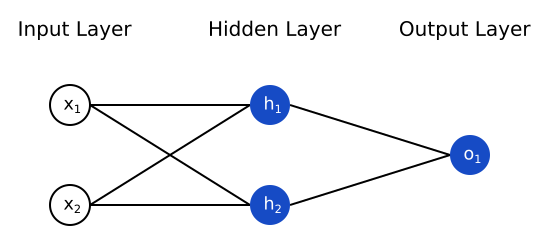
\includegraphics[width=0.5\textwidth]{./img/neural-network}
			\caption{Red neuronal simple con dos entradas y una salida.}
			\label{neural-network}
		\end{figure}
	
		Como podemos observar en dicha figura \ref{neural-network}, la red consta de una capa de entrada con dos neuronas, una red intermedia con otras dos, y finalmente de la capa de salida. Debemos saber que en dicha capa intermedia es donde se realizan sobre los datos de entrada todas las operaciones matemáticas que comentábamos anteriormente.\\
		
		Además, ha de destacarse que la conexión entre las neuronas de la red viene determinada por unos \textbf{pesos numéricos característicos}. Estos pesos son los que se utilizan a la hora de hacer el cálculo de salida final, dando una mayor importancia a ciertas neuronas con respecto a otras.\\
		
		Finalmente, en la capa de salida se combinan como entradas las salidas de la capa intermedia para, mediante una \textbf{función de activación}, producir una determinada salida.
		
	\subsection{Redes neuronales para tratamiento de imágenes}
	
		Conociendo las redes neuronales simples, debemos saber que \textbf{no son apropiadas para su uso con imágenes} debido a lo siguiente \cite{intro-convolutional-nn}:
		
		\subsubsection*{Tamaño de las imágenes}
		
			Los píxeles de una imagen son los que han de introducirse como entradas a la primera capa de una red neuronal. Si una imagen consta de 150 píxeles en blanco y negro, existirán 150 entradas. Si la imagen es a color (en modo \textit{RGB}), el número de entradas se multiplican por los tres canales de dicho formato.\\
			 
			Esto quiere decir que si una imagen consta de millones de píxeles, como encontramos actualmente en las tomadas por un teléfono móvil cualquiera, tendríamos que entrenar \textbf{millones de pesos} en la primera capa, lo que es prácticamente imposible en cualquier ordenador del que dispongamos.
			 
		\subsubsection*{Posición de las imágenes}
		
			Aunque en dos imágenes se muestre el mismo objeto para cuya detección ha sido entrenada la red neuronal simple, con una de este tipo no se es capaz de detectar que dicho objeto pueda cambiar en el espacio mostrado por la imagen. Es decir, aunque aparezca la misma cara humana que en otra imagen antes estudiada, que este elemento cambie de posición en la imagen implica que no sean las mismas neuronas las que se activen, por lo que el resultado de salida puede (y con mucha probabilidad) no ser el esperado.
			
		\subsubsection*{Solución}
		
			La solución para estos problemas la encontramos en las \textbf{redes neuronales de tipo convolucional}, que no son más que redes simples como las ya estudiadas pero que utilizan unas capas especiales, llamadas \textit{convolucionales}.\\
			
			Una \textbf{convolución} no es más que un filtro aplicado de forma iterativa a la imagen en forma de pequeña matriz de dos dimensiones. Un ejemplo práctico lo podemos ver en la referencia \cite{intro-convolutional-nn}, que aplica un \textbf{filtro horizontal de \textit{Sobel}} para mostrar la detección de límites en una imagen.\\
			
			En este caso el filtro usado (o \textit{kernel}) se muestra en la figura \ref{conv-filter}. Adicionalmente, en la figura \ref{conv-filter-result} se visualizan a la izquierda la imagen original sobre la que se aplica el filtro, y a su derecha la imagen resultante. Como podemos ver, el resultado es una nueva fotografía en blanco y negro donde se manifiestan los límites más relevantes de dicha foto.\\
			
			\begin{figure}[h]
				\centering
				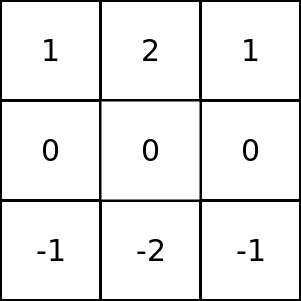
\includegraphics[width=0.2\textwidth]{./img/horizontal-sobel}
				\caption{Ejemplo de matriz de convolución - Filtro horizontal de \textit{Sobel}.}
				\label{conv-filter}
			\end{figure}
		
			\begin{figure}[h]
				\centering
				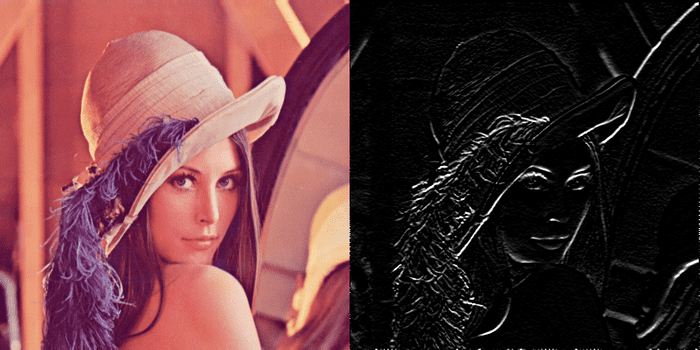
\includegraphics[width=0.6\textwidth]{./img/lenna+horizontal}
				\caption{Imagen original y su resultante tras aplicar el filtro convolucional de \textit{Sobel}.}
				\label{conv-filter-result}
			\end{figure}
		
			Utilizando la detección de límites de forma previa al entrenamiento de la red, se delimitan mucho mejor los elementos contenidos en la imagen, por lo que se favorece mucho dicha fase de aprendizaje.
	
	\subsection{\textit{Deep Learning}}
	
		Se conoce como \textbf{aprendizaje profundo} al campo de aplicación del \textbf{aprendizaje automático} donde se hace un uso más extenso de técnicas basadas en \textbf{redes neuronales artificiales}. Estas redes utilizadas son capaces de aprender \textit{profundamente} para trabajar con problemas como reconocimiento de imágenes, de texto o de voz; además de otras aplicaciones como filtrado colaborativo en redes sociales y visión por computador.\\
		
		La diferencia principal entre una red neuronal simple y las redes de \textit{aprendizaje profundo} reside en que las primeras, como ya hemos visto anteriormente, contienen una suma de tres capas: la de \textbf{entrada}, la \textbf{intermedia} (donde se aplican las operaciones) y la de \textbf{salida}.\\
		
		Por otro lado, en las redes neuronales de \textit{deep learning} el número de capas intermedias es mayor, con lo que se consigue un mejor aprendizaje. Esto se debe a que el número de neuronas (y por tanto de pesos en el modelo final) es mayor; y cuanto más alto sea el número de hiperparámetros presentes en un algoritmo, mayor es la capacidad de entrenamiento que tendrá dicho modelo final.\\
		
		\begin{figure}[h]
			\centering
			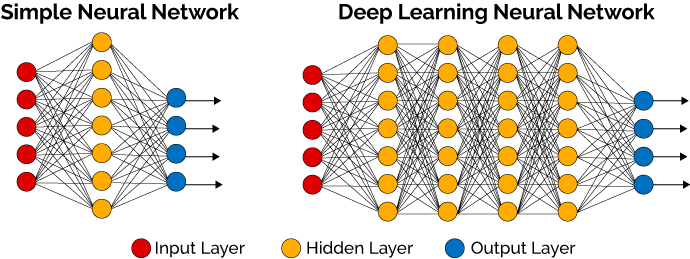
\includegraphics[width=0.8\textwidth]{./img/neural-network-differences}
			\caption{Diferencia entre red neuronal simple y red de aprendizaje profundo.}
			\label{nn-differences}
		\end{figure}
	
		\subsubsection*{Clasificación categórica}
		
			La finalidad de cualquier técnica de clasificación (o \textit{clustering}) es lógicamente asignar una clase concreta a cada una de las entradas. Esta clasificación podría ser \textbf{binaria} (si existen tan solo dos clases) o \textbf{multicategórica} (si existen más de dos).\\
			
			El problema de las clasificaciones multicategóricas es que pueden no detectar demasiado bien las características de cada clase y el modelo resultante puede errar con alta frecuencia en sus predicciones. Este problema también se evidencia con la existencia de un desequilibrio en el número de datos de cada clase encontrados en la fase de entrenamiento.\\
			
			Una forma de intentar poner solución a este problema es el uso de \textit{técnicas de binarización}, las cuales comentaremos en el apartado siguiente.
	
		\subsubsection{Técnicas de binarización}
		
			Al igual que en los métodos del tipo \verb|"divide y vencerás"|, surgen como técnica basada en la descomposición de un problema en otros de menor dimensión, de forma que en un problema de \textit{clustering}, no encontramos más de dos clases a la vez (clasificación binaria). Como podría esperarse, surge la necesidad de combinar las distintas salidas de cada uno de los nuevos clasificadores para así realizar la predicción final de clase (lo que se conoce como \textbf{agregación}). Veremos las técnicas de agregación más adelante.\\
			
			Según podemos ver en la referencia \cite{binary-classifiers}, artículo escrito por un grupo de investigación de profesores de nuestra propia facultad, existen dos técnicas de binarización principales: \textit{\textbf{One-vs-One}} y \textit{\textbf{One-vs-All}}, que describimos a continuación:\\
			
			{\large \textbf{\textit{One-vs-One}}}: Se basa en el uso de un clasificador binario para discriminar entre un par de clases. El conjunto de datos utilizado para entrenamiento es el subconjunto del \textit{dataset} donde se encuentra asignada una de las dos clases, ignorando así los datos que pertenecen a las otras categorías. En la gráfica \ref{one-vs-one} se puede ver una representación gráfica de la técnica descrita.\\
			
			La clase de salida suele decidirse por algún modelo basado en votación, donde cada clasificador vota por una clase preferida y la asignada finalmente es aquella con mayor número de votos.\\
			
			\begin{figure}[h]
				\centering
				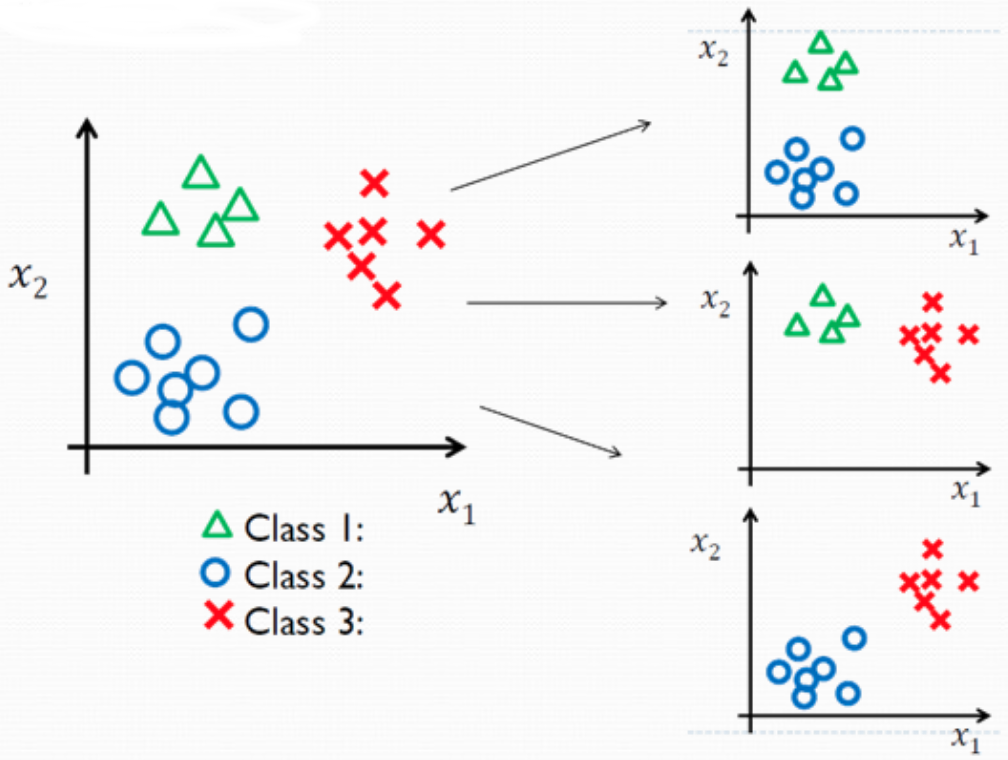
\includegraphics[width=0.6\textwidth]{./img/one-vs-one}
				\caption{Ilustración de las comparaciones uno a uno de cada modelo. \cite{binarization-slides}}
				\label{one-vs-one}
			\end{figure}
			
			{\large \textbf{\textit{One-vs-All}}}: Se reduce el problema a tantos problemas binarios como clases existan, donde en cada uno de ellos se realiza el enfrentamiento entre una sola clase y el grupo de categorías compuesto por el resto. En la gráfica \ref{one-vs-all} se puede ver una representación gráfica de la técnica descrita.\\
			
			En este caso los datos de entrenamiento usados se corresponden con los del \textit{dataset} completo, considerando de la categoría \textit{positiva} los de la clase única, y como \textit{negativa} los del resto.\\
			
			\begin{figure}[h]
				\centering
				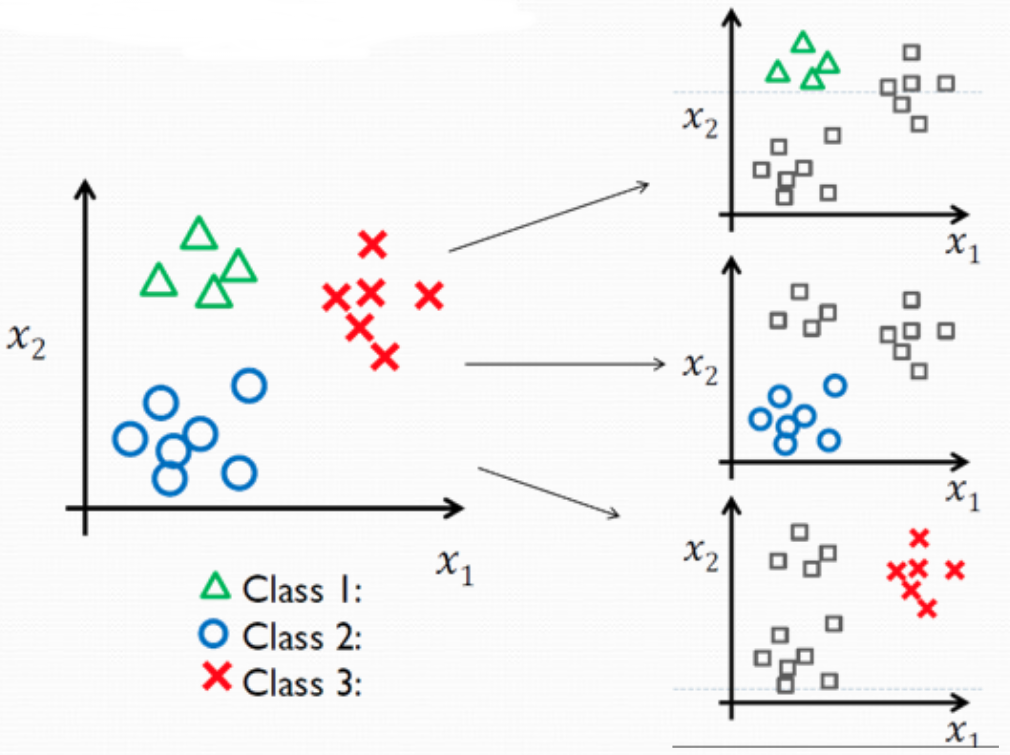
\includegraphics[width=0.6\textwidth]{./img/one-vs-all}
				\caption{Ilustración de las comparaciones uno contra el resto de cada modelo. \cite{binarization-slides}}
				\label{one-vs-all}
			\end{figure}
			
			Como ya adelantábamos, una vez que disponemos de distintos clasificadores que resuelven problemas más pequeños, se requiere de una gestión de las múltiples salidas para su integración en una sola etiqueta, es decir, la categoría decidida finalmente para la entrada inicial. Pasemos por tanto a comentar las técnicas de agregación que ponen solución a esto.
			
		\subsubsection{Técnicas de agregación (\textit{Ensembles})}
		
			Como venimos adelantando, consisten en la integración de múltiples salidas de pequeños clasificadores para la decisión de una sola. Como mencionan en la referencia \cite{ensembling-methods}, un ejemplo sería el de un proceso de contratación para un demandante de empleo, donde la decisión final de su incorporación reside en el acuerdo entre todos los entrevistadores.\\
			
			Podemos encontrar distintos tipos, entre los que destacamos los siguientes:
			
			\begin{itemize}
				\item \textbf{Estrategia basada en votación}: es quizá la más sencilla. Cada clasificador vota por una categoría, se realiza un recuento y aquella clase que haya recibido más votos es la decidida finalmente por el modelo para la entrada dada.
				\item \textbf{Estrategia basada en votación con pesos}: sigue la idea anterior pero en este caso cada clasificador asigna una clase con un determinado peso, en función de la confianza que tiene en dicha predicción.
				\item \textbf{\textit{Boosting}}: se trata de una técnica secuencial donde el primer algoritmo es entrenado contra el \textit{dataset} completo. Una vez que el algoritmo ha realizado la clasificación, se toman todos los datos que han sido categorizados de forma errónea, y el siguiente algoritmo intenta clasificarlos correctamente. Se repite este comportamiento para los algoritmos subsecuentes.
			\end{itemize}
		
			En nuestro caso, más adelante comentaremos con más detalle la estrategia basada en \textbf{votación con pesos}, que será la que utilicemos para intentar mejorar el rendimiento de nuestro trabajo desarrollado para el apartado de investigación.
		
\section{Desarrollo de la práctica}

	Una vez que hemos hecho una puesta en contexto de algunas de las técnicas que utilizaremos para el desarrollo del proyecto, es momento de ponernos manos a la obra con la aplicación de redes neuronales de distintos tipos, poniendo en práctica lo aprendido hasta el momento.\\
	
	Como mencionamos en la introducción, utilizaremos el \textit{dataset} de predicción de tiempo de adopción de animales; que cargaremos en diferentes tipos de redes neuronales con los distintos \textit{tunings} que apliquemos. Sobre estas redes, utilizaremos distintas métricas que nos guiarán hacia la persecución del mejor resultado que podamos obtener. Respecto a estas métricas, debemos hacer algunas apreciaciones iniciales:\\
	
	{\large \textbf{\textit{Accuracy}}}: prestaremos especial atención a este valor, el cual traducimos por \verb|"precisión"|. Este evalúa directamente el porcentaje de aciertos del modelo de predicción con respecto al número de elementos. En las conclusiones realizaremos algunos comentarios al respecto pero, por ahora, quedemos con que un \textbf{clasificador aleatorio} a priori deberá tener un porcentaje de precisión igual a 100 dividido entre el número de clases. Dicho esto, sabremos que en este problema que estamos tratando gozaremos de un \textit{accuracy} inicial del 20\% (100 entre las 5 categorías).\\
	
	{\large \textbf{\textit{Loss}}}: se trata de un valor \textit{perjudicial} que pretendemos minimizar al máximo. Cuanto mayor sea, significará que las predicciones se alejan más de lo que sería la clasificación ideal. En el apartado de conclusiones también realizaremos algunas apreciaciones adicionales, pero debemos tener presente que se deben estudiar las dos métricas de forma conjunta.\\
	
	Antes de entrar en materia, examinemos en forma de histograma la distribución de los datos del \textit{dataset} en las distintas categorías. Esto puede verse en la figura \ref{histogram}. En dicha imagen se pone de manifiesto el \textbf{gran desbalanceo existente entre las clases} que encontramos, sobretodo en la primera (que recordemos que representa el menor tiempo de adopción predicho para los animales).\\
	
	\begin{figure}[h]
		\centering
		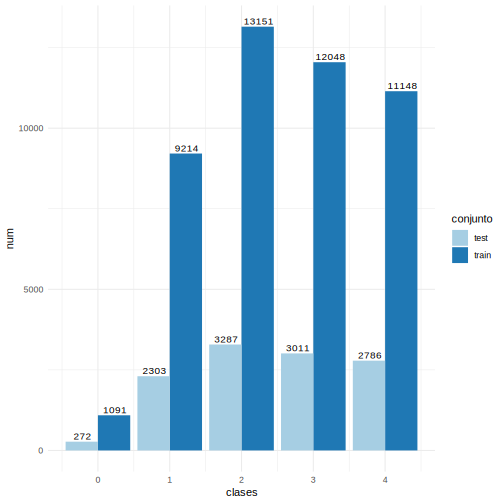
\includegraphics[width=0.85\textwidth]{./img/bp_dataset_particionado}
		\caption{Cardinales de los subconjuntos de cada clase del \textit{dataset}.}
		\label{histogram}
	\end{figure}

	Para finalizar con el planteamiento de la práctica, hemos \textbf{particionado el conjunto} de datos en dos: un primer subconjunto que sirve para el entrenamiento y la validación de los modelos, conteniendo el \textbf{80\%} de los datos totales; y un segundo subconjunto que contiene el resto de datos, y cuya finalidad es evaluar la generalización y el rendimiento de dichos modelos.\\ 
	
	Una vez visto esto, pasemos a ver primeramente la red más básica, inspirada en lo aprendido en clase.

	\subsection{Primera aproximación - Red vista en clase}
	
		Se utiliza la misma red neuronal vista en las prácticas de la asignatura y accesible desde el repositorio correspondiente del profesor \cite{red-clase}.\\
	
		Consta de una arquitectura muy típicamente vista en problemas de reconocimiento de imágenes a través del uso de redes neuronales. La estructura viene dada por la utilización de convoluciones y aplicaciones de \textit{pooling}; que sirve para concentrar en un solo píxel un conjunto cuadrado de estos, y así reducir la dimensión de la matriz estudiada, dado que la aplicación de convoluciones hace que crezca.\\
		
		Como en todas las redes que utilizaremos, disponemos de \textbf{cinco neuronas} para la capa de salida (tantas como categorías manejadas).\\
		
		En la figura \ref{first-nn} podemos visualizar un gráfico con el resultado del entrenamiento del modelo, junto con la representación de su validación con el conjunto de datos correspondiente.\\
	
		\begin{figure}[h]
			\centering
			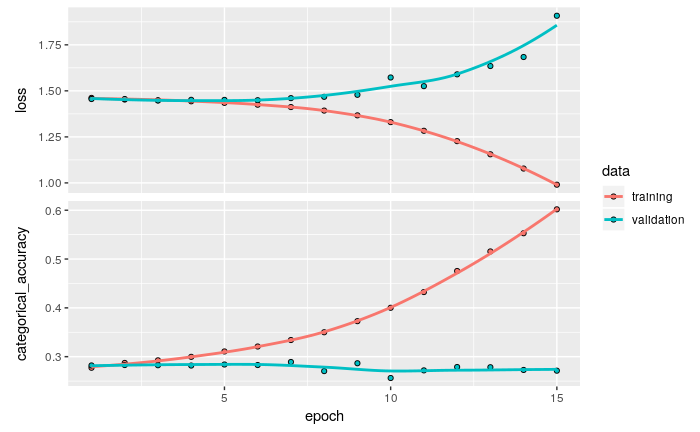
\includegraphics[width=0.9\textwidth]{./img/model1}
			\caption{Gráfica resultado del entrenamiento del primer modelo.}
			\label{first-nn}
		\end{figure}
	
		En dicha figura, para los distintos subconjuntos de datos (entrenamiento y validación), podemos apreciar varias cosas:
		
		\begin{itemize}
			\item Fase de \textbf{entrenamiento}: conforme el número de épocas aumenta, el valor de \textit{accuracy} crece y el de \textit{loss} disminuye. Esto es lo esperado, ya que manifiesta el aprendizaje de la red neuronal sobre los datos presentados en el entrenamiento, aumentando su precisión y disminuyendo el número de errores de predicción.
			\item Con respecto a la \textbf{validación}: se puede ver claramente que la \textit{precisión} se mantiene constante, mientras que el número de errores crece. Esto evidencia dos cosas: \begin{itemize}
				\item Los datos aprendidos por la red durante el entrenamiento no tienen correlación alguna con los contenidos en el subconjunto de validación, y por ello no se altera el primer valor.
				\item El algoritmo está \textit{sobreaprendiendo}; es decir, ajustándose demasiado a los datos aprendidos y no generalizando correctamente sobre aquellos nuevos que no conoce.
			\end{itemize}
		\end{itemize}
	
		A modo de última apreciación, debemos saber que el valor de \textit{\textbf{accuracy}} en el conjunto de evaluación es de \textbf{28,43\%}, valor aproximado al que decíamos que contendría un clasificador aleatorio; y que su valor de \textbf{pérdida} es de \textbf{1,45}.
		
	\subsection{Segunda aproximación - Balanceo de clases}
	\label{balanceo-clases-subsection}
	
		Como veíamos en la figura \ref{histogram}, el desbalanceo encontrado en los datos es muy acentuado, lo que será perjudicial para las clases minoritarias, que tendrán una menor presencia en la fase de entrenamiento del modelo, quien predirá de forma favorable a las clases mayoritarias.\\
		
		Para evitar esto, se asignan \textbf{pesos} a las clases en función de los cardinales de cada categoría para intentar equilibrarlos. Como podría esperarse, los pesos serán mayores en las clases minoritarias y menores en el resto, de forma proporcional al número de datos.\\
		
		Estos pesos se relacionan con el algoritmo de aprendizaje en la función de pérdida del mismo, ya que éste siempre intenta minimizar dicha función. Las clases minoritarias tienen un peso mayor que el resto, por lo que pueden anteponerse de esta forma a otras categorías que teóricamente deberían tener más representación. Esto puede provocar un número mayor de errores o unas predicciones aún más alejadas de la realidad, disparando así el valor de \textbf{\textit{loss}}.\\
		
		En la figura \ref{second-nn} podemos visualizar un gráfico con el resultado del entrenamiento del modelo, junto con la representación de su validación con el conjunto de datos correspondiente.\\
	
		\begin{figure}[h]
			\centering
			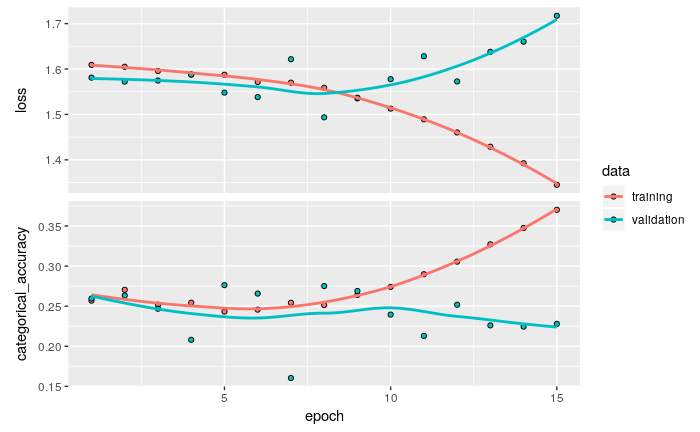
\includegraphics[width=0.9\textwidth]{./img/model2}
			\caption{Gráfica resultado del entrenamiento del segundo modelo.}
			\label{second-nn}
		\end{figure}
	
		Como se puede observar, su valor de \textbf{precisión} de partida es menor al del primer modelo. Al igual que sucedía en dicho modelo, el algoritmo comienza a sobreaprender, esta vez en torno a la décima época. En este momento se aprecia que el valor de pérdida del subconjunto de validación comienza a aumentar claramente. Al igual que sucedía en el modelo anterior, es entonces cuando el valor de precisión del subconjunto de entrenamiento se distancia considerablemente del de validación, y su pérdida empieza a disminuir.\\
		
		En este modelo se consigue un \textbf{\textit{accuracy}} de \textbf{23,21\%} frente a un valor \textbf{\textit{loss}} de \textbf{1,66}. Fácilmente podemos determinar que este modelo ofrece un resultado peor que el anterior, acercándose aún más al 20\% de un clasificador aleatorio. 
	
	\subsection{Tercera aproximación - \textit{Data augmentation}}
	
		Para este caso práctico, a las imágenes existentes en nuestro caso de estudio les vamos a aplicar diversas transformaciones para crear otras nuevas, y así gozar de un \textbf{número mayor de muestras} para el entrenamiento. Las utilizadas han sido las siguientes: rotación aleatoria de en torno a 30 grados, volteado horizontal y/o vertical.\\
		
		Si bien el número inicial de imágenes era de \textbf{X}, tras este proceso de aumento de muestras disponemos de un total de \textbf{Y} fotografías; lo que teóricamente podría ayudarnos a aumentar la generalización y rendimiento de nuestro modelo, disminuyendo también los errores. Veremos a continuación si conseguimos el resultado esperado.\\
				
		En la figura \ref{third-nn} podemos visualizar un gráfico con el resultado del entrenamiento del modelo, junto con la representación de su validación con el conjunto de datos correspondiente.\\
	
		\begin{figure}[h]
			\centering
			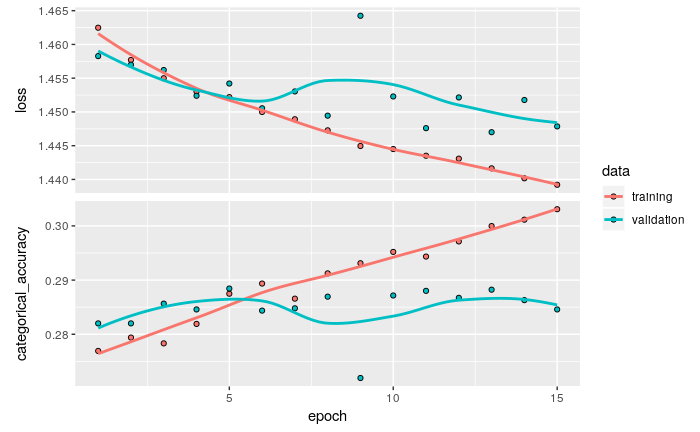
\includegraphics[width=0.9\textwidth]{./img/model3}
			\caption{Gráfica resultado del entrenamiento del tercer modelo.}
			\label{third-nn}
		\end{figure}
	
\section{Trabajo de investigación}

	De forma adicional a la práctica desarrollada, hemos querido centrar nuestra investigación en las técnicas de binarización mencionadas en el marco teórico explicado anteriormente en este documento, realizando varias ejecuciones prácticas y aportando las conclusiones extraídas de dicho trabajo.\\
	
	Particularmente, optamos por la implementación de técnicas \textbf{\textit{One-vs-one}} y \textbf{\textit{One-vs-all}}, también descritas anteriormente. Sabemos que disponemos de 5 categorías en las que clasificar los datos por lo que podemos predecir que en el primer caso dispondremos de 10 modelos, y de 5 en el segundo. Además, de forma proactiva, hemos decidido realizar pruebas de ambas técnicas de forma dual, tanto con los datos sin balancear como con ellos balanceados. Veremos los resultados obtenidos en las siguientes subsecciones.\\
	
	De forma previa a su explicación, cabe destacar que el balanceo utilizado en los próximos modelos es igual al utilizado en la sección \nameref{balanceo-clases-subsection}.

	\subsection{\textit{One-vs-one} sin balancear}
	
		Para empezar, nos encontramos con los 10 modelos generados por el enfrentamiento uno-a-uno entre las 5 clases existentes en el \textit{dataset}. Cabe recordar que al encontrarnos enfrentando solamente dos clases, el clasificador aleatorio toma un valor de \textit{accuracy} del \textbf{50\%}. A continuación, en el cuadro \ref{ovo-sin-balanceo} podemos encontrar una tabla con los resultados.\\
	
		\begin{table}[h]
			\centering
			\resizebox{\textwidth}{!}{%
				\begin{tabular}{lllllllllll}
					\multicolumn{1}{c}{} & 0 vs 1     & 0 vs 2     & 0 vs 3     & 0 vs 4     & 1 vs 2     & 1 vs 3     & 1 vs 4     & 2 vs 3     & 2 vs 4     & 3 vs 4     \\ \hline
					loss                 & 0.3481 & 0.2762 & 0.2932 & 0.2874 & 0.7930 & 0.8128 & 0.8359 & 0.9399 & 0.7924 & 0.8011 \\
					acc                  & 0.8943 & 0.9235 & 0.9165 & 0.9136 & 0.5286 & 0.5557 & 0.5829 & 0.5247 & 0.5625 & 0.5524
				\end{tabular}%
			}
			\caption{Tabla de resultados de los modelos \textit{One-vs-one} sin balanceo de datos.}
			\label{ovo-sin-balanceo}
		\end{table}
	
		Los resultados obtenidos son similares para algunos casos, por lo que comentaremos los más representativos. Por ejemplo, podemos encontrar un valor de \textit{accuracy} muy alto para la comparación entre la clase 0 y el resto (en torno al 90\%), véase figura \ref{ovo-01}. Esto es debido a que la clase 0, como sabemos, tiene un cardinal de datos muy bajo (clase \textbf{minoritaria}) mientras que sus \textit{rivales} constan de muchos más datos. Es por esto que, si el clasificador solamente clasifica correctamente los datos de las clases rivales, erra en muy pocas ocasiones (los datos de la clase 0 no penalizan demasiado), dejando un valor final alto.\\
		
		En cambio, si nos fijamos en el valor \textit{accuracy} de la comparación entre el resto de clases ronda el 50\%, lo cual denota una \textbf{clasificación aleatoria} pero donde existe un balanceo más equitativo de los datos (véase figura \ref{ovo-23}).\\
	
		\begin{figure}[h]
			\centering
			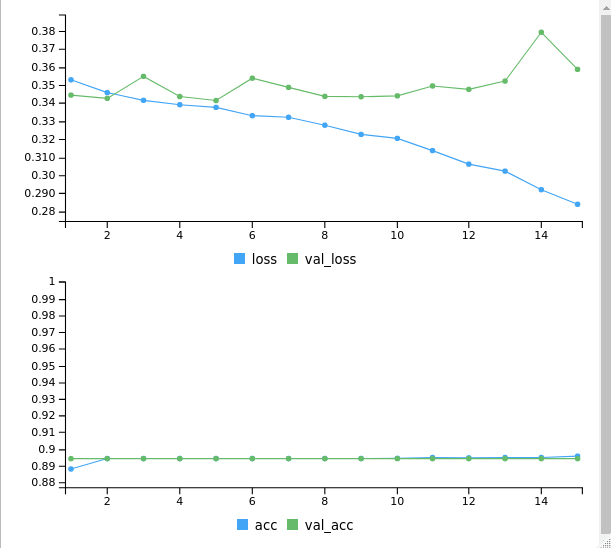
\includegraphics[width=0.6\columnwidth]{./img/OVO_01}
			\caption{Modelo de predicción generado por \textbf{clase 0} vs. \textbf{clase 1} (\textit{One-vs-one} sin balanceo).}
			\label{ovo-01}
		\end{figure}
	
		\begin{figure}[h]
			\centering
			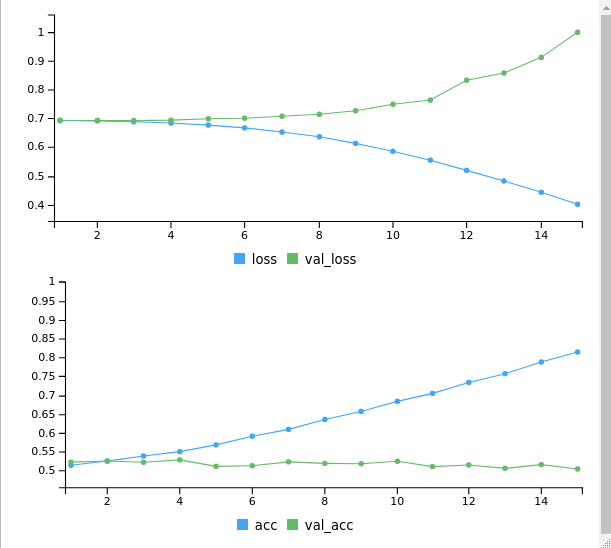
\includegraphics[width=0.6\columnwidth]{./img/OVO_23}
			\caption{Modelo de predicción generado por \textbf{clase 2} vs. \textbf{clase 3} (\textit{One-vs-one} sin balanceo).}
			\label{ovo-23}
		\end{figure}
	
	\subsection{\textit{One-vs-one} balanceado}
	
		En este caso, aplicamos sobre el caso práctico anterior un balanceo basado en \textbf{pesos}, como explicábamos en la sección \nameref{balanceo-clases-subsection}. Además, debemos saber que seguimos teniendo 10 modelos y que el porcentaje de precisión del clasificador aleatorio es del 50\%. A continuación encontramos en el cuadro \ref{ovo-con-balanceo} una tabla con los resultados obtenidos tras las ejecuciones.\\
	
		\begin{table}[h]
			\centering
			\resizebox{\textwidth}{!}{%
				\begin{tabular}{lllllllllll}
					\multicolumn{1}{c}{} & 0 vs 1     & 0 vs 2     & 0 vs 3     & 0 vs 4     & 1 vs 2     & 1 vs 3     & 1 vs 4     & 2 vs 3     & 2 vs 4     & 3 vs 4     \\ \hline
					loss                 & 0.5259 & 0.5165 & 0.5786 & 0.5641 & 0.8058 & 0.7883 & 0.7757 & 0.8466 & 0.7972 & 0.7887 \\
					acc                  & 0.7373 & 0.7223 & 0.6776 & 0.6932 & 0.5340 & 0.5481 & 0.5636 & 0.5266 & 0.5635 & 0.5572
				\end{tabular}%
			}
			\caption{Tabla de resultados de los modelos \textit{One-vs-one} con balanceo de datos.}
			\label{ovo-con-balanceo}
		\end{table}
	
		El cambio significativo que apreciamos tras la aplicación de pesos con respecto a su predecesor sin balanceo reside en la comparativa entre la clase 0 y el resto; ya que el valor de \textit{accuracy} baja notablemente en casi un 20\%, mientras que para el resto de comparativas entre clases no tan minoritarias se mantienen los valores en torno al 50\%.\\
		
		Este descenso se debe a la penalización en la función de \textit{pérdida} del algoritmo de aprendizaje. Podríamos extraer una conclusión errónea al pensar que la clase 0 se distingue mejor del resto dado que comporta un valor de \textit{precisión} mayor, pero esto puede deberse al bajo volumen de datos donde la población es poco representativa y se hallan muchas similitudes entre ellos.\\
		
		Más adelante, en las figuras \ref{ovo-bal-01} y \ref{ovo-bal-23} pueden encontrarse las mismas comparaciones mostradas para el modelo anterior. De la primera podemos decir que el valor de precisión vuelve a mantenerse constante durante el aprendizaje pese a que el valor de pérdida disminuye. Por el contrario, en la fase de validación ambos valores se comportan de forma prácticamente aleatoria, no siguiendo ningún patrón.\\
		
		En la segunda imagen podemos ver que el valor de \textit{accuracy} aumenta durante el entrenamiento progresivamente, debido a que el valor de pérdida en este caso disminuye; mientras que en la etapa de validación el primer valor no se altera en todo el proceso, si bien el segundo aumenta notablemente con respecto a su valor durante el entrenamiento.\\
	
		\begin{figure}[h]
			\centering
			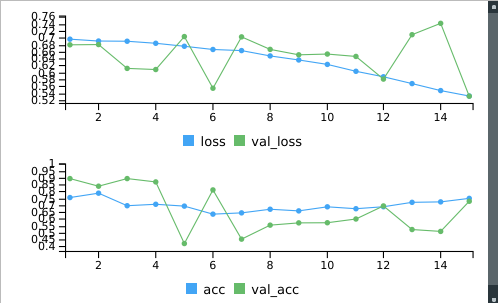
\includegraphics[width=0.6\columnwidth]{./img/OVO_bal_01}
			\caption{Modelo de predicción generado por \textbf{clase 0} vs. \textbf{clase 1} (\textit{One-vs-one} con balanceo).}
			\label{ovo-bal-01}
		\end{figure}
		
		\begin{figure}[h]
			\centering
			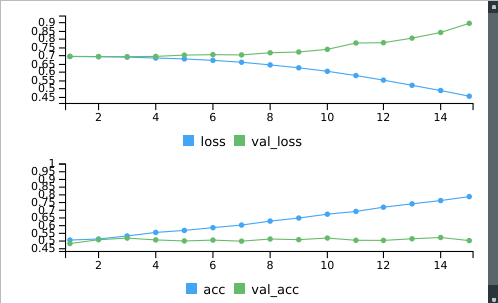
\includegraphics[width=0.6\columnwidth]{./img/OVO_bal_23}
			\caption{Modelo de predicción generado por \textbf{clase 2} vs. \textbf{clase 3} (\textit{One-vs-one} con balanceo).}
			\label{ovo-bal-23}
		\end{figure}
		
	\subsection{\textit{One-vs-all} sin balancear}
	
		Como anticipábamos, estos modelos se basarán en el enfrentamiento entre cada una de las clases con respecto al conjunto formado por el resto. Es importante decir que en esta metodología el desbalanceo intrínseco de los datos es aún más acentuado y acuciante que anteriormente.A continuación encontramos en el cuadro \ref{ova-sin-balanceo} una tabla con los resultados obtenidos tras las ejecuciones.\\
			
		\begin{table}[h]
			\centering
			\begin{tabular}{llllll}
				     & 0      & 1      & 2      & 3      & 4      \\ \hline
				loss & 0.1556 & 0.5016 & 0.6651 & 0.6049 & 0.5717 \\
				acc  & 0.9761 & 0.8015 & 0.6707 & 0.7248 & 0.7271
			\end{tabular}%
			\caption{Tabla de resultados de los modelos \textit{One-vs-all} sin balanceo de datos.}
			\label{ova-sin-balanceo}
		\end{table}
	
		En dicha tabla, podemos ver que en la clase minoritaria encontramos un altísimo valor de \textit{accuracy} y uno de \textit{loss} muy bajo, lo que teóricamente debería ser positivo pero que viene dado por el desbalanceo antes mencionado. En el resto, encontramos valores más cercanos entre sí, de un 70\% para la precisión y de 0.55 para la pérdida.\\
		
		Cabe destacar que la clase 2, siendo la mayoritaria, aquí tiene el menor \textit{accuracy}, lo que pone de manifiesto que al compararse con la suma de todos sus rivales, el desequilibrio de cardinales de clases es menor.\\
	
		\begin{figure}[h]
			\centering
			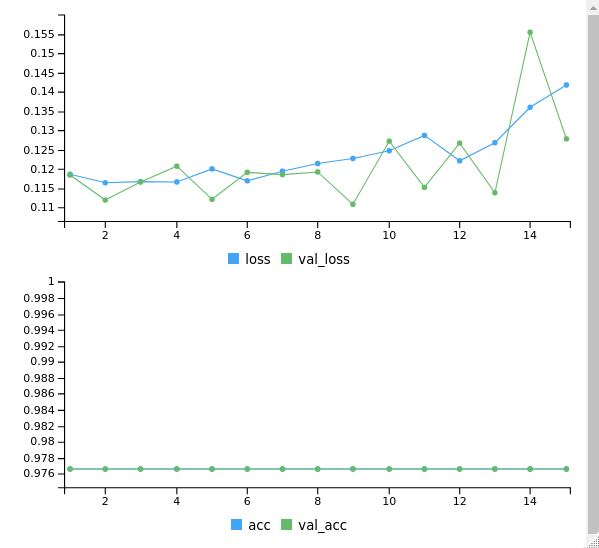
\includegraphics[width=0.6\columnwidth]{./img/OVA_0}
			\caption{Modelo de predicción generado por \textbf{clase 0} (\textit{One-vs-all} sin balanceo).}
			\label{ova-0}
		\end{figure}
		
		\begin{figure}[h]
			\centering
			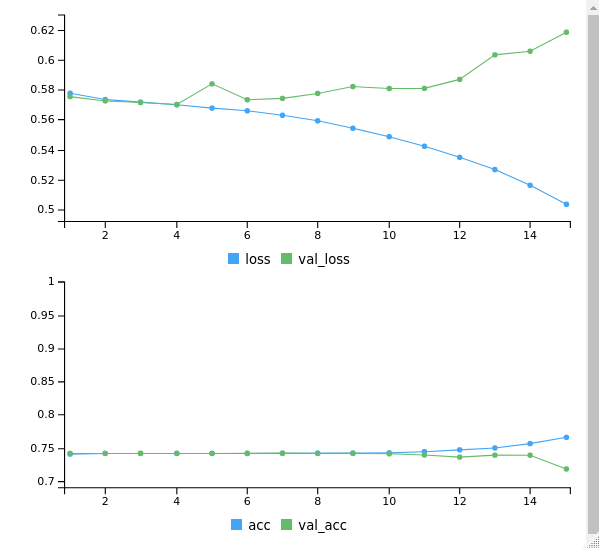
\includegraphics[width=0.6\columnwidth]{./img/OVA_3}
			\caption{Modelo de predicción generado por \textbf{clase 3} (\textit{One-vs-all} sin balanceo).}
			\label{ova-2}
		\end{figure}
	
		En la figura \ref{ova-0} podemos ver el resultado del enfrentamiento entre la clase 0 y sus rivales, (es decir, la ejecución con mayor desbalanceo). En ella podemos apreciar también que el valor de \textit{accuracy}, que es alto por los motivos ya expuestos anteriormente, también se mantiene constante, una vez más debido a su bajo cardinal de elementos.\\
	
	\subsection{\textit{One-vs-all} balanceado}
	
		Para finalizar con la aplicación de técnicas de binarización, llegamos a la utilización de la metodología \textit{One-vs-all} una vez más, esta vez usando de nuevo el balanceo basado en pesos previamente mencionado.\\
		
		En el cuadro \ref{ova-con-balanceo} encontramos la tabla con los resultados obtenidos. En ella podemos observar cómo el valor de precisión se mantiene prácticamente igual que su predecesor sin balanceo; mientras que el valor de pérdida aumenta muy considerablemente para la clase minoritaria, pero se mantiene constante para el resto.\\
		
		Al igual que en la modalidad \textit{One-vs-one} con balanceo, aquí la función de pérdida vuelve a influenciarse por los pesos aplicados sobre las clases. Este comportamiento se acentúa aún más en la función de \textit{loss} de la clase 0 (la minoritaria, como sabemos), pasando de tener un valor 0,15 en la modalidad sin balanceo a un 0,51 en este caso; aunque realmente el de \textit{accuracy} no se vea afectado.\\
	
		\begin{table}[h]
			\centering
			\begin{tabular}{llllll}
				     & 0      & 1      & 2      & 3      & 4      \\ \hline
				loss & 0.5120 & 0.6498 & 0.6638 & 0.6448 & 0.5946 \\
				acc  & 0.9753 & 0.7719 & 0.6127 & 0.7360 & 0.7301
			\end{tabular}%
			\caption{Tabla de resultados de los modelos \textit{One-vs-all} con balanceo de datos.}
			\label{ova-con-balanceo}
		\end{table}
	
		\begin{figure}[h]
			\centering
			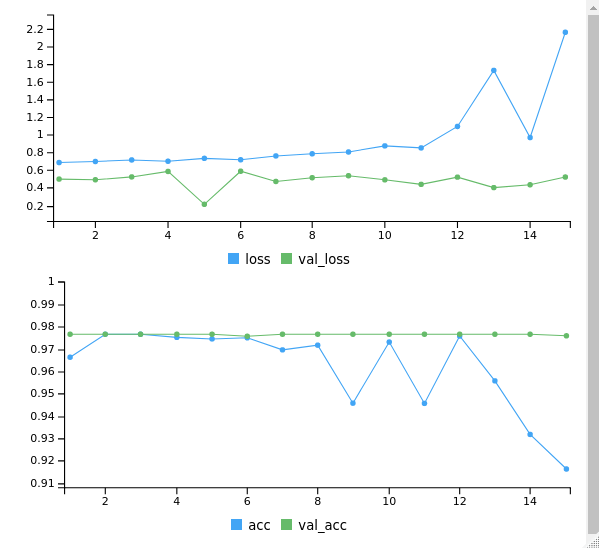
\includegraphics[width=0.6\columnwidth]{./img/OVA_bal_0}
			\caption{Modelo de predicción generado por \textbf{clase 0} (\textit{One-vs-all} con balanceo).}
			\label{ova-bal-0}
		\end{figure}
		
		\begin{figure}[h]
			\centering
			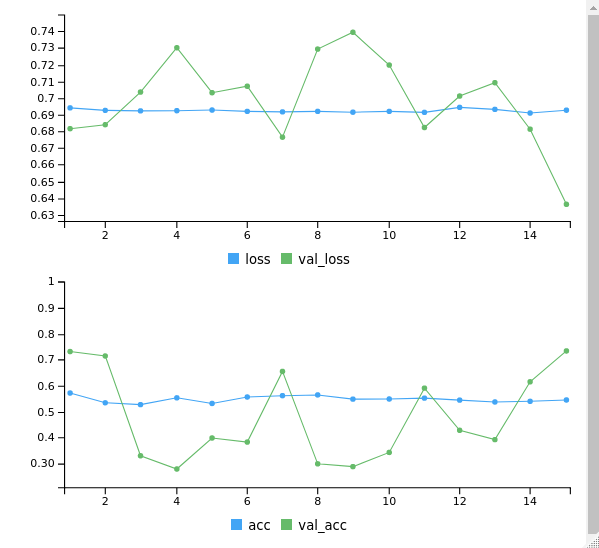
\includegraphics[width=0.6\columnwidth]{./img/OVA_bal_3}
			\caption{Modelo de predicción generado por \textbf{clase 3} (\textit{One-vs-all} con balanceo).}
			\label{ova-bal-3}
		\end{figure}
		
	\subsection{\textit{Ensembling} de los modelos desarrollados}
	
		Como anticipábamos en el marco teórico de las \textit{técnicas de binarización}, surge la inmediata necesidad de realizar una agregación de los distintos modelos clasificadores binarios para disponer finalmente de uno solo que maneje toda la información generada por sus antecesores; y que sea éste quien realice finalmente la predicción multicategórica.\\
		
		Para visualizar un caso práctico basado en esta técnica, nuestra idea se basaba en realizar una pequeña red neuronal densa que concentrase a modo de entradas las salidas de dichos modelos, y que la salida generada por ésta fuese una de las clases comprendidas entre 0 y 4, traducible directamente por el tiempo de adopción que llevaría a una familia para rescatar a uno de los animales del centro sobre el que trata el problema.\\
		
		Realmente, lo que estaríamos generando de ser así sería una agregación de redes que siguiese la \textbf{estrategia de votación por pesos}, donde cada uno de los pequeños modelos de clasificación binaria aportarían un peso en función de la confianza que tienen sobre su predicción. Los hiperparámetros internos de esta red (es decir, los pesos que unen las neuronas de la capa de entrada con la de salida), se corresponden con los pesos de dicha estrategia por votación, pero que son calculados de forma automática.\\
		
		Sin embargo, pese a haber realizado pequeñas pruebas relacionadas con esto, no hemos sabido finalmente como integrar estos modelos \textit{OvO} y \textit{OvA} de forma exitosa en una red neuronal más sencilla y contenida. Aún así, en el fichero fuente (\verb|.Rmd|) aportado junto con este documento para la práctica, se puede ver el código utilizado para dichas pruebas.
		
	\subsection{Modelo probado de Internet}
	
		Para complementar con el número de pruebas realizado para el trabajo, se ha probado también la red neuronal descrita en el enlace web de la referencia \cite{cbonett-cnn}. En el ejemplo encontrado en el artículo de dicha web, se realiza una \textbf{clasificación de artículos \textit{e-Commerce} basada en el análisis de imágenes y texto}, por lo que pensamos que sería de gran ayuda para encontrar un modelo de predicción provechoso y que dotase de buen rendimiento.\\
		
		Cabe destacar que dicha red se encuentra programada en el lenguaje \textit{Python} utilizando \textit{keras}, la misma librería que utilizamos en \textit{R} para la creación de redes neuronales. Sin embargo, pasar esta red de \textit{Python} a \textit{R} \textbf{no fue tan sencillo como esperábamos}, y una vez más tras realizar diversas pruebas y dedicarle unas horas de tiempo, no conseguimos que el ejemplo funcionase correctamente, si bien el código también se adjunta dentro del fichero fuente aportado con la práctica.\\
		
		Esta red consta de 13 capas de convolución, por lo que se podría esperar que extrajera un mayor volumen de características a cambio de un entrenamiento más costoso (debido al mayor número de pesos que entrenar). Sin embargo, también nos atrevemos a anticipar que por muchas capas de convolución que se añadan, no se puede extraer de las imágenes más información de la que hay, por lo que \textbf{el resultado no llegaría a ser mucho mejor}, si bien nuestra intención inicial era comprobarlo de forma empírica.
	
\section{Conclusiones}

	Aunque ya hemos ido realizando una discusión de resultados extensa durante la obtención y representación de los modelos, para cerrar el trabajo hemos de plantear algunas conclusiones finales que manifiestan lo aprendido durante \textit{el trayecto}.
	
	\begin{itemize}
		\item Como venimos diciendo a lo largo del documento, \textbf{el valor de \textit{accuracy} ha de ser analizado muy detenidamente y confrontado con otras métricas}. Encontrar un valor muy alto aquí no quiere decir que el modelo tenga un rendimiento excelente y muy generalizado, sino que puede deberse a causas como el desbalanceo de los datos, al igual que hemos visto a lo largo del trabajo de investigación.
		\item En este caso, las imágenes utilizadas para el aprendizaje de las redes \textbf{no aportan la información suficiente} para el problema que se quiere tratar. Es decir, ¿realmente se puede predecir de forma eficaz el tiempo que tardará una familia cualquiera en adoptar a un perro simplemente con su aspecto? Intervienen muchos otros factores más llamativos para la gente como la raza, la edad y su historial de vacunas, entre otros. Sin embargo, todos estos atributos son muy difícilmente reconocibles para nuestra red.
		\item Como venimos poniendo de manifiesto, el \textbf{desbalanceo de los datos} de cada clase que usamos para entrenar hace que el modelo no sea lo suficientemente generalizado y que por tanto no responda bien ante datos nuevos no conocidos.
		\item Además, las \textbf{técnicas de binarización} utilizadas no dotan del comportamiento esperado, dado que les afectan los problemas ya mencionados como el desequilibrio y la poca información que extraemos de las imágenes encontradas.
	\end{itemize}

	En resumen, el principal problema del \textit{dataset} utilizado reside en utilizar tanto las imágenes usadas como los datos numéricos, ya que como hemos dicho, las fotografías por sí solas no aportan información suficiente para la resolución del problema planteado.\\

	Para terminar, cabe decir que esto comporta el final de un \textbf{trabajo muy interesante e ilustrativo} sobre las técnicas encontradas en la asignatura; que nos ha servido para presenciar en primera plana los retos y dificultades que sufre un problema de ciencia de datos real, donde los \textit{datasets} no tienen porqué estar balanceados y los recursos de los que disponemos (en este caso imágenes) pueden no ser productivos para la resolución.\\
	
	Es por este motivo por lo que antes de enfrentarnos a un problema de ciencia de datos, se debe realizar un \textbf{estudio efusivo y detallado} de los mismos, así como tener un breve conocimiento del reto encontrado en sí antes de abordarlo; para prever problemas de viabilidad además de realizar alguna selección y eliminado previo de características que no aportan información a dicho problema.

\newpage
\bibliographystyle{plain}
\bibliography{sources}

\end{document}
